\section{Die Regeln}
\label{Regeln}
Diese Arbeit beschäftigt sich nur mit der meist verbreiteten Art von Sudokus. Dabei spielt man auf einem 9x9 Felder großen Spielfeld, das wiederum in neun 3x3 Felder große Blöcke eingeteilt ist. Weiter handelt es sich nur dann um ein Sudoku, wenn genau eine Lösung vorhanden ist.
Ein Sudoku gilt dann als gelöst, wenn jede Zeile, jede Spalte und jeder Block die Ziffern 1 bis 9 genau einmal enthält.
\begin{figure}[h]
\begin{center}
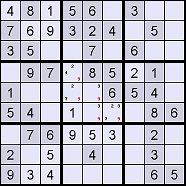
\includegraphics{./img/sudoku.jpg}
\caption{Sudoku}
\end{center}
\end{figure}



Ein Sudoku hat immer eine eindeutige Lösung, sonst ist es kein Sudoku.